\documentclass[main.tex]{subfiles}
\begin{document}

\textbf{Exercise 1. Fermat's Principle}\\
\textbf{Q\&A} Lifeguard Alice can run at speed $v_r$ on the beach and swim at speed $v_s$ in the water, with $v_r > v_s$. What is the path (Determined by Alice starting angle $\theta_i$ in \textbf{Equation \ref{sol1a}}) that minimizes the time for reaching point B and saving Bob from drowning?\\

\begin{figure}
\centering\fbox{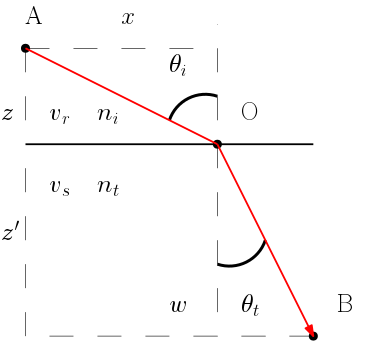
\includegraphics[height=2.0in]{figures/hw1_1.png}}
\caption{Path traveled by Alice \textbf{A} to reach Bob \textbf{B} which minimizes travel time.}
\label{fig:1}
\end{figure}

We know that $v_r > v_s$ and $\therefore$ we know that $n_i < n_t$ and \\

$\because$ the velocity of light (life guard Alice) and material index are inversely related as follows:  $n_i = c / v_r$ and $n_t = c / v_s$ and \\

$\because$ Snell's law states the relationship between the incident index and angle and the transmission index and angle is defined as: $n_i\sin(\theta_i) = n_t \sin(\theta_{t})$ where we know that when light is traveling from a lower to higher index, towards optically denser material, the transmission angle $\theta_t$ with respect to normal decreases, resulting in the maximum incident angle ($\theta_i = 90$ degrees) that can enter the optically dense medium: $n_i = n_t \sin(\theta_t)$\\

$\therefore$ we can state that $\frac{c}{v_r} = \frac{c}{v_s} \sin(\theta_t)$ and $\therefore$ that $v_s = v_r \sin(\theta_t)$\\

$\because$ Trigonometrically we know that $\sin(\theta_i) = \frac{x}{\sqrt{x^2 + z^2}}$\\


$\because$ the Path the light  (aka lifeguard Alice), shown in Figure \ref{fig:1},  travels  = $AO + OB = n_i \sqrt{(x^2 + z^2)} + n_t \sqrt{(w-x)^2 +  z^{\prime 2}}$ and\\

$\because$ the Shortest Path is determined by setting the derivative equal to zero such that $ \frac{\partial \text{Path}}{\partial x} = n_i \frac{x}{\sqrt{(x^2 + z^2)}} - n_t \frac{w-x}{\sqrt{((w-x)^2 + z^{2\prime 2})}} = 0$ which trigonometrically we know is equivalent to $n_i \sin{\theta_i} - n_t \sin{\theta_t} = 0$\\

When we rewrite in terms of velocity and set equal we arrive at $\frac{c}{v_r}\sin{\theta_i} = \frac{c}{v_s} \sin{\theta_t}$ and simplify $v_s\sin{\theta_i} = {v_r}\sin{\theta_t}$ and $\therefore$ we have shown that in order to take the path of least resistance and minimize time light (and the lifeguard) will run at an angle normal to the beach equal to 

\begin{equation}\label{sol1a}
\theta_i = \arcsin{(\frac{v_r}{v_s} \sin{\theta_t})}
\end{equation}

\textbf{Exercise 2. Total Internal Reflection}\\
\textbf{Q\&A} Derive the critical angle $\theta$ (Equation \ref{eq:2a}) for which total internal reflection happens at the first interface (core-cladding). Hint: Both Fermat's principal and Snell's law are accepted for the derivation. What is the numerical aperture (Equation \ref{eq:2b}) of the fiber? Assuming a GRIN from 1.5 to 1.4 what is the trajectory (Qualitatively Sinusoidal) of the ray in case of total internal reflection ? \\

\begin{figure}
\centering\fbox{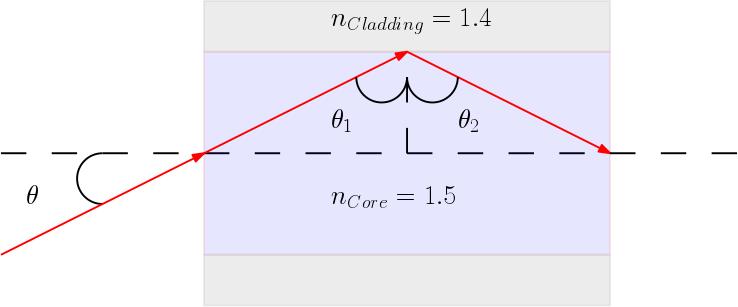
\includegraphics[height=2.0in]{figures/hw1_2.png}}
\caption{Required $\theta$ in Equation \ref{eq:2a} for total internal reflection to occur}
\label{fig:2}
\end{figure}

\textbf{Big Fat Assumption:} Ray entering cladding does not change ray trajectory, even though going form $n_{Air} = 1$ into $n_{Core} = 1.5$\\

\textbf{Snells Law} for Total Internal Reflection $n\sin(\theta_i) = n^{\prime}\sin(\theta_{ref})$\\

The Critical angle $\theta_c$ of the incident ray results in a refracted ray that travels parallel to the materials interface. For the \textbf{generic} problem with a interface between a material with index of refraction n and air with index of refraction 1, Snell's Law becomes, using radians, $n\sin(\theta_c) = 1\sin(\pi/2)$ which simplifies to $n\sin(\theta_c) = 1$. This signifies that for total internal reflection to occur in the \textbf{generic}  $n\sin(\theta_c) > 1$. \\

We can adapt the \textbf{generic} problems critical angle condition $n\sin(\theta_c) = 1\sin(\pi/2)$ with the \textbf{current} problems given material index's resulting in  $1.5\sin(\theta_1) = 1.4\sin(\theta_2 = \pi/2)$. Mapping from the \textbf{generic} problem we know that for total internal reflection to occur $1.5\sin(\theta_1) > 1.4\sin(\theta_2 = \pi/2)$ which simplifies to $\theta_1 > \arcsin(\frac{1.4}{1.5})$.\\

Invoking our \textbf{Big Fat Assumption} and utilizing trigonometry's similar angles, utilizing radians, we know that $\pi/2 = \theta  + \theta_1$. Understanding that $\theta$ will be a positive angle off of our normal axis, we know that for total internal reflection to occur $\pi/2 - \theta > \arcsin(\frac{1.4}{1.5})$. We can solve for $\theta$ by multiplying by $-1$, showing us that for total internal reflection to occur 

\begin{equation}\label{eq:2a}
\theta < \pi/2 - \arcsin(\frac{1.4}{1.5})
\end{equation}

The numerical aperture is the incident angle of acceptance of the fiber, generally stated as $(\text{NA}) \equiv \sin(\theta_0) \leq \sqrt{n_1^2 - n_2^2}$, or referencing figure \ref{fig:2} and explicitly stated for our problem as $(\text{NA}) \equiv \sin(\theta) \leq \sqrt{1.5^2 - 1.4^2}$, resulting in 

\begin{equation}\label{eq:2b}
(\text{NA}) \leq 0.5385
\end{equation}

For a Fiber with a GRIN (Gradient Index) between $n_{max} = 1.5$ and $n_{min} = 1.4$, if the condition $n_{max}\sin(\theta_0)$ is respected, light in a uniform medium propagates in a straight line where as light in a gradient fiber propagates along a \textbf{sinusoidal} path.\\

\textbf{Exercise 3. Ellipsoidal refractor}\\
\textbf{Q\&A} What is the dimension of the axes of an ellipsoidal refractor $(n=1.5)$ which focuses a plane wave ($\lambda_1 = \SI{1.55e-6}{\meter}$) impinging on axis (rays parallel to the major axis) in its focal point $f =  \SI{2.5e-2}{\meter}$? Would the same refractor perfectly focus at wavelength $\lambda_2 = \SI{0.5e-6}{\meter}$ considering that the refractive $n$ index varies to $1.6$? If yes why? If no, which would be the dimension of the ellipse that focuses it? Would the the ellipsoidal refractor be affected by any kind of aberration? Motivate your answer. Graduate Students: Additional point if you can use any ray tracing software for demonstrating the functioning of the refractor.\\

\begin{figure}
\centering\fbox{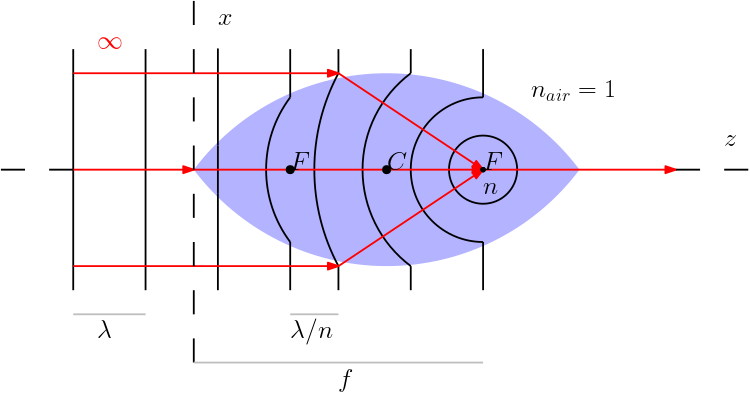
\includegraphics[height=2.0in]{figures/hw1_3.png}}
\caption{Ellipsoidal refractor}
\label{fig:3}
\end{figure}

The dimension of the $x$ axes of an ellipsoidal refractor when focusing a object at $\infty$, with rays parallel to the major $z$ axes, to an image at $F$, is defined by the ellipsoidal refractor equation $\left(s-\frac{n}{n+1}f \right)^2 + \frac{n^2}{n^2 - 1}x^2 = \left(\frac{n}{n+1}f \right)^2$ where $s=\frac{x^2}{4f}$. When solving for $x$ we see that the solution is independent of wavelength $\lambda$.\\

\begin{equation}
\left(\frac{x^2}{4f}-\frac{n}{n+1}f \right)^2 + \frac{n^2}{n^2 - 1}x^2 = \left(\frac{n}{n+1}f \right)^2
\end{equation}

\textbf{Exercise 4. Hyperboloidal refractor}\\

\textbf{Q\&A} Prove that a hyperbolodial refractor is an ideal refractor that can convert a spherical wave into a planar wave, or in other words image at infinity a point object.\\

\begin{figure}
\centering\fbox{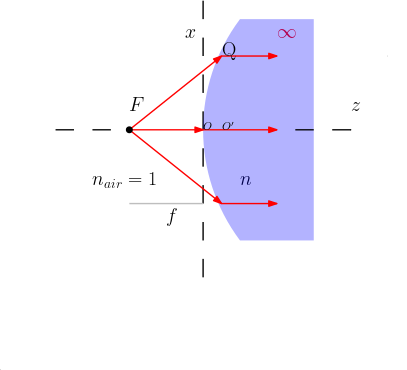
\includegraphics[height=2.0in]{figures/hw1_4.png}}
\caption{Hyperboloidal refractor}
\label{fig:4}
\end{figure}

$FQ = FO + nOO^{\prime}$ $\because$ rays on differing trajectories must travel the same distance.\\

$\therefore \sqrt{(f+s)^2 + x^2} = f + ns$  and\\ 

$\therefore  f^2+ 2fs + s^2 + x^2 = f^2 + 2nfs + n^2s^2$  and\\ 

$\therefore 2fs + s^2 + x^2 = 2nfs + n^2s^2$  and\\ 

$\therefore x^2  - s^2(n^2 - 1) - 2fs(n- 1) = 0$  and divide by $(n^2 - 1)$ \\ 

$\therefore \frac{1}{n^2 - 1} x^2  - s^2 - 2fs(\frac{1}{n + 1}) = 0$  and \\ 

$\therefore  - s^2 - 2fs(\frac{1}{n + 1}) = -\frac{1}{n^2 - 1} x^2 $  and \\ 

$\therefore  - s^2 - 2fs(\frac{1}{n + 1}) = -\frac{1}{n^2 - 1} x^2 $  and \\ 

$\therefore  0 = s(s + 2f(\frac{1}{n + 1})) -\frac{1}{n^2 - 1} x^2 $  and \\

$\therefore \left(s-\frac{1}{n+1}f \right)^2 - \frac{1}{n^2 - 1}x^2 = \left(\frac{1}{n+1}f \right)^2$ \\

\textbf{Exercise 5. Immersed lens}\\

\text{Q\&A} A lens (refractive index $n_0$ with a left curvature $R_1$ and a right curvature $R_2$) is immersed in two different liquids $n_1$ and $n_2$. Under the paraxial assumption determine the focal length and power of the lens. Hint: Use ray transfer matrix. Assuming that the lens is in air, and has a focal length of $\SI{1.0e-2}{\meter}$. The object has an elevation $h_1=1$ is positioned at $\SI{5.0e-2}{\meter}$ away from the lens. What is the lateral magnification? What is the distance?

%The ideal imaging element is referred to as asphere, or as ashperic lens. It works perfectly on axis and reasonably well in a limited range of angles off-axis. A Non Perfect Image results from a non planar wave front generated by spherical aberration. 

\begin{equation}\label{eq:5a}
n_{Left} \alpha_{Left} = n_{Right} \alpha_{Right} - \frac{n_{Left} - n_{Right}}{R}x
\end{equation}

\begin{figure}
\centering\fbox{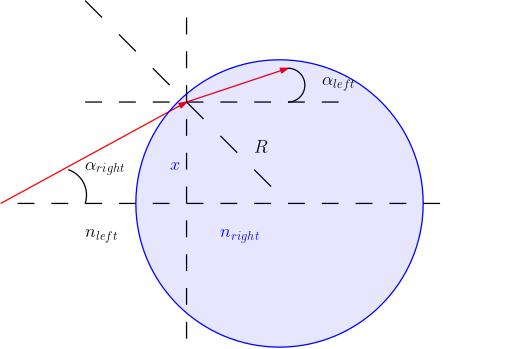
\includegraphics[height=2.0in]{figures/hw1_5b.png}}
\caption{Spheric Paraxial Assumption Variables Spatial Relationships}
\label{fig:5b}
\end{figure}

Equation \ref{eq:5a} referencing figure \ref{fig:5b} defines the trajectory of a light ray in a sphere. Assuming that $\sin(\alpha_{right}) << 1$, and that $\sin(\alpha_{left}) << 1$, the paraxial approximation requires that $x<<R$. Height $x$ of the material index interface on the light ray refraction trajectory is by definition spatially equal on both sides of the interface, expresses as $ x_{left}=x_{right}$. The change in index, change in trajectory relationship within a spherical lens can be expressed by the following ray transfer matrix\\

\begin{pmatrix}
    n_{right} \alpha_{right} \\
    x_{right}
\end{pmatrix}
=
\begin{pmatrix}
    1   & -\frac{n_{right}-n_{left}}{R} \\
    0   &   1
\end{pmatrix}
\begin{pmatrix}
    n_{left}\alpha_{left} \\
    x_{left}
\end{pmatrix}\\

We can trace the trajectory of light passing along a cascade of optical elements under the paraxaial assumption, assuming the assumption holds at each change in index of refraction interface.\\

The thin lens approximations spatial relationships noted in figure \ref{fig:5c} define $t=R-R\cos{\phi}= 2R\sin^2\phi$ where the parazial approximation assumes that $\alpha_{max} << 1$ and $\therefore$ $\phi_{Max} << 1$ and $\therefore$ thickness $t \approx 0$.\\ 

\begin{figure}
\centering\fbox{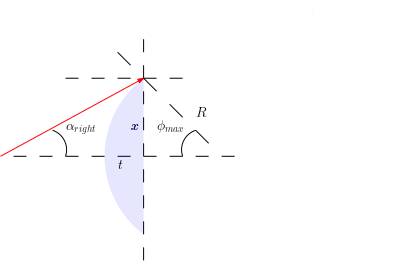
\includegraphics[height=2.0in]{figures/hw1_5c.png}}
\caption{Thin Lens Approximation Variables Spatial Relationships}
\label{fig:5c}
\end{figure}

The a focus of the bundle or rays diverging from point source $S$ referenced in \ref{fig:5d} forms a diverging spherical waves emanating from height $h_0$ above the $z$ axis within liquid $1$s index of refraction $n_1$ refract into the thin spherical lens with left curvature $R_1$, index of refraction $n_0$, while traveling as a non perfect collimated beam, before reaching the lens right curvature $R_2$ and refracting into liquid $2$s index of refraction $n_2$ and converging as a spherical wave to height $h_1$ bellow the $z$ axis at point $P$. The system is said to be stigmatic for points $S$ and $P$ with $P$ referred to as a perfect image of $S$.\\ In an ideal optical system, these conjugate points will be stigmaticlly (perfectly) imaged.

It is important to note that both $\alpha_1$ and $\alpha_2$ are both negative angles due to their clockwise orientation,that $h_1$ is negative due to its down ward orientation bellow the $z$ axis, and that both $R_1>0$ and $R_2>0$ in a Bi convex lens.\\

$V_1$ is the vertex of the surface, and $\bar{}$ The length $s_0$ is know as the object distance, and the \\

The ray transfer matrix between the $n_1$, $n_0$ interface, is defined as\\

\begin{bmatrix}
    n_{0} (-\alpha_{1}) \\
    (h_{0})
\end{bmatrix}
=
\begin{bmatrix}
    1   & -\frac{n_{0}-n_{1}}{R_1} \\
    0   &   1
\end{bmatrix}
\begin{bmatrix}
    n_{1} (-\alpha_{1}) \\
    h_{0}
\end{bmatrix}\\

The ray transfer matrix between the $n_1$, $n_0$ interface, and the $n_0$, $n_2$ interface is defined as\\

\begin{bmatrix}
    n_{2} (-\alpha_{2}) \\
    (-h_{1})
\end{bmatrix}
=
\begin{bmatrix}
    1   & -\frac{n_{2}-n_{0}}{R_2} \\
    0   &   1
\end{bmatrix}
\begin{bmatrix}
    1   & -\frac{n_{0}-n_{1}}{R_1} \\
    0   &   1
\end{bmatrix}
\begin{bmatrix}
    n_{1} (-\alpha_{1}) \\
    h_{0}
\end{bmatrix}\\

which simplifies to\\

Stuck on how to properly add off axis object to matrix form\\

\begin{figure}
\centering\fbox{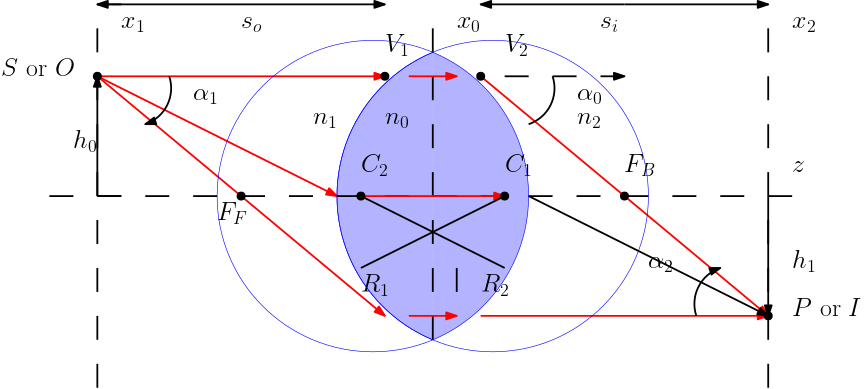
\includegraphics[height=2.0in]{figures/hw1_5a.png}}
\caption{Immersed Bi-convex lens image formation at finite distances variables spatial relationships}
\label{fig:5d}
\end{figure}


\end{document}
